\documentclass[12pt, openany]{report}
\usepackage[utf8]{inputenc}
\usepackage[T1]{fontenc}
\usepackage[a4paper,left=2cm,right=2cm,top=1cm,bottom=2cm]{geometry}
\usepackage[french]{babel}
\usepackage{libertine}
\usepackage[pdftex]{graphicx}
\usepackage[export]{adjustbox}
\usepackage{setspace}
\usepackage{hyperref}

\hypersetup{
    colorlinks=true,
    linkcolor=blue,
    filecolor=magenta,      
    urlcolor=cyan,
}
\setstretch{1,4}
\setlength{\parindent}{4ex}
\setlength{\parskip}{1ex plus 0.5ex minus 0.2ex}
\newcommand{\hsp}{\hspace{20pt}}
\newcommand{\HRule}{\rule{\linewidth}{0.5mm}}

\begin{document}
\begin{titlepage}
  \begin{sffamily}
  \begin{center}

	\begin{figure}[t]
	   \begin{minipage}{0.48\textwidth } 
	     
\includegraphics[width=.3\linewidth , left]{ensias.JPG}
	   \end{minipage}\hfill
	   \begin{minipage}{0.48\textwidth }
	     
\includegraphics[width=.4\linewidth , right]{univesite.JPG}
	   \end{minipage}
	\end{figure}
     
    \textsc{\LARGE École nationale supérieure d'informatique et d'analyse des systèmes}\\[4cm]


    % Title
    \HRule \\[0.5cm]
    { \huge \bfseries Présentation du sujet de projet de fin d'année: Crop Mapping\\[0.4cm] }
	\HRule\\[4cm]

    % Author and supervisor
    \begin{minipage}{0.4\textwidth}
      \begin{flushleft} \large
        \emph{Réalisé par:}\\
        AIT LAHCEN \textsc{Ahmed}\\
	CHICHI \textsc{Hamza}\\
       \emph{Filière, Groupe}\\
	Génie logiciel, GL 1\\
      \end{flushleft}
    \end{minipage}
    \begin{minipage}{0.4\textwidth}
      \begin{flushright} \large
       \emph{Sous la direction de:}\\
	Mme. Sanaa. \textsc{EL FKIHI}\\
	\end{flushright}
    \end{minipage}

    \vfill

    % Bottom of the page
    {\large Année universitaire 2019/2020}

  \end{center}
  \end{sffamily}
\end{titlepage}
\newpage
\strut 

\listoffigures
\tableofcontents
\chapter{Présentation du sujet}

\section{Les parcelles}

\subsection{Définition de parcelle}
Une parcelle est généralement une superficie de terrain ayant une unité de propriété. Une parcelle peut être dans ce cas la propriété d'une personne privée ou publique, seule ou en groupe.
Un ensemble de parcelles peut être désigné comme un « parcellaire ». 
\begin{figure}[hp]
\centering
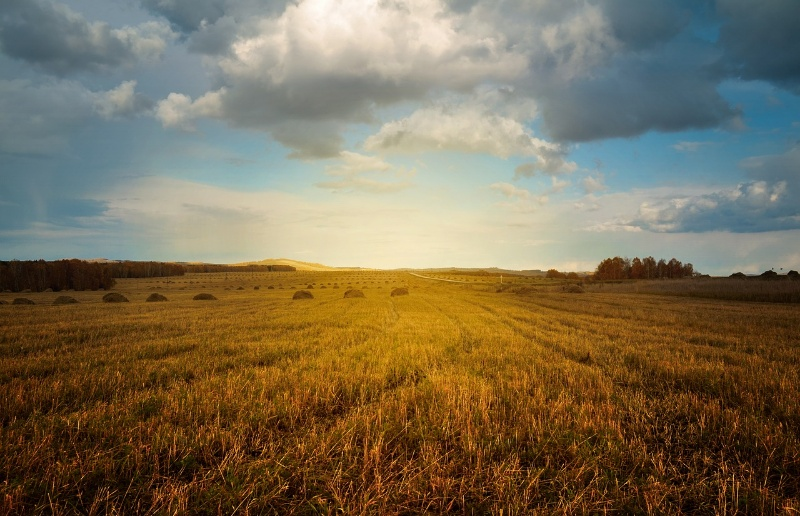
\includegraphics[scale=0.5]{parcelle2.jpg}
\caption{Une parcelle}
\end{figure}
Selon le référentiel foncier ou d'organisation spatiale utilisé, le terme de parcelle peut s'appliquer à différents domaine :\\
•	en agriculture, elle désigne alors la division agricole (champ, pré, vignoble, verger, etc.) exploitée par la même personne ou le même groupe de personnes.\\
•	en sylviculture, G. Sêe, sous-inspecteur des forêts définissait les parcelles en 18681 comme des « enceintes formées par des lignes de configuration, de fertilité ou de consistance » en préférant ce mot à l'ancien mot de « canton » qu'il considère même comme un néologisme quand on le réutilise (à cette époque).\\
•	en urbanisme et dans les plans cadastraux, elles sont définies selon leurs propriétaires et leurs limites parcellaires, tant en milieu rural qu'urbain. Ainsi, une parcelle définit autant une unité de terrain agricole, qu'un terrain habité, ou encore une parcelle à l'abandon ou dévolue aux stationnements automobiles.  \hyperref[sec:refs]{1}
\subsection{La segmentation des parcelles}
La fragmentation des parcelles a des intérêts agronomique et écologique, Une largeur moyenne des parcelles, inférieure à 150 mètres, permet une diffusion efficace des insectes auxiliaires des cultures depuis les bordures de champ.
Les carabes, prédateurs des limaces, sont des auxiliaires de référence. Il est admis que depuis une bordure de champ, ils pénètrent au maximum jusqu’à 75 mètres à l’intérieur de la parcelle.
\begin{figure}[hp]
\centering
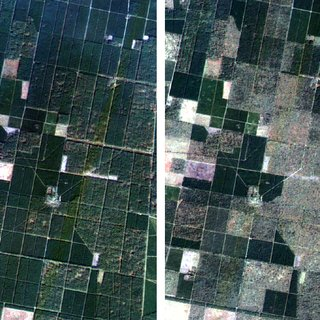
\includegraphics[scale=1]{seg.jpg}
\caption{La fragmentation d'une parcelle}
\end{figure}
De manière générale, conserver des parcelles culturales de petite taille augmente l'hétérogénéité du paysage.
Du point de vue agronomique, la propagation de maladies, ravageuses et parasites est contenue.
Du point de vue écologique:\\
•	le paysage est plus diversifié\\
•	L’effet de lisière est augmenté \hyperref[sec:refs]{2}
\subsection{Les type de culture sur une parcelle}
En fonction de la productivité, différents systèmes de production agricole sont définis :\\
• l’agriculture intensive ou productiviste qui est caractérisée par l’usage important d’intrants et cherche à maximiser la production par rapport aux facteurs de production, qu’il s’agisse de la main d’œuvre, du sol ou des autres moyens de production (matériel, intrants divers).\\
• l’agriculture extensive qui ne maximise pas la productivité du sol et ne fait pas appel à des intrants chimiques, à l’arrosage ou au drainage, mais plutôt aux ressources naturellement présentes sur place. Pratiquée généralement sur de vastes étendues, elle se caractérise par des rendements à l’hectare relativement faibles.\\
• l’agriculture vivrière ou de subsistance est une forme d’agriculture qui consiste à cultiver des produits essentiellement destinés à nourrir la population localement. \hyperref[sec:refs]{3} 
\begin{figure}[hp]
\centering
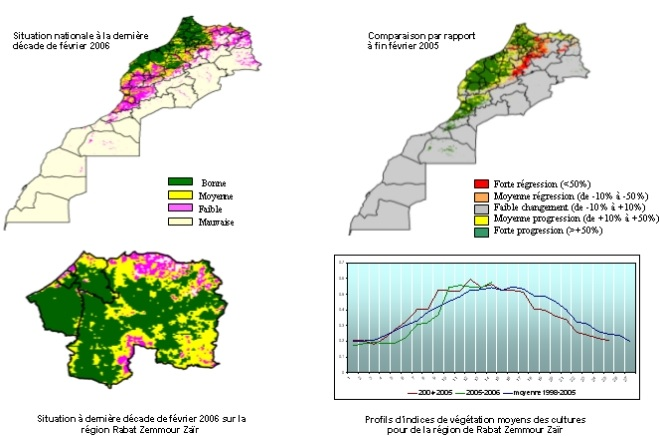
\includegraphics[scale=0.9]{etat.jpg}
\caption{L'état des cultures au maroc}
\end{figure}\\
Les modes de culture les mieux connus sont l’agriculture conventionnelle et l’agriculture biologique. Face à la volonté de préserver l’environnement et l’évolution des pratiques, des types d’agriculture alternative se sont mises en place : l’agriculture durable, l’agriculture raisonnée, l’agriculture intégrée, l’agriculture multifonctionnelle, l’agriculture de précision. Dernièrement, un mode de culture qui se pratique en dehors du sol est apparu : l’agriculture hors-sol ou hydroponie.
\hyperref[sec:refs]{4}
\section{Les images satellites}
\subsection{La définition d'une image satellite}
Une image satellite, ou image satellitaire, est une prise de vue transmise d'un satellite artificiel en orbite. Elles permettent d'obtenir différentes informations comme la surveillance des pays ennemis pour les militaires (fonction première de la création d'un satellite d'observation), prévisions météorologiques (par exemple les satellites Météosat), ou tout simplement pour les recherches sur l'Univers. Certains satellites sont capables d'une précision telle que cela peut devenir un problème, notamment en termes de vie privée ou de secret d'État. \hyperref[sec:refs]{5}
\begin{figure}[hp]
\centering
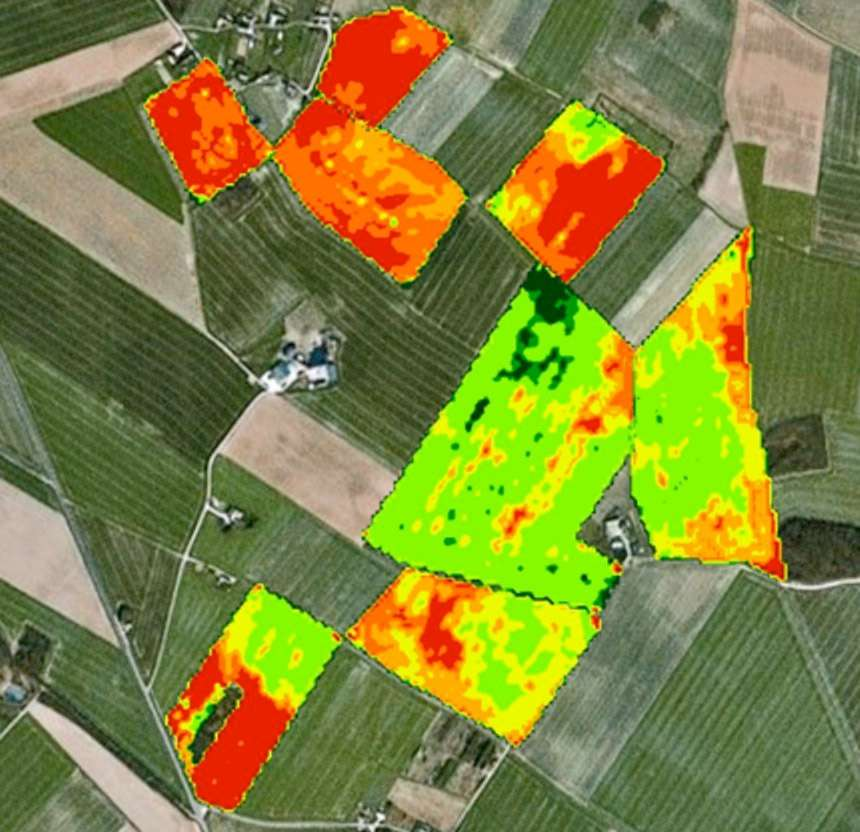
\includegraphics[scale=0.5]{img.jpg}
\caption{Image d'une parcelle par satellite}
\end{figure}

\subsection{Les satellites au service de l'agriculture}
Dans le domaine de l'agriculture, les satellites d'observation de la Terre sont utilisés pour une très grande variété d’applications et de services, comme la surveillance des cultures, le contrôle des surfaces et de l'occupation des sols, l'irrigation et la des gestion des cultures en engrais et produits phytosanitaires. Ils sont également utilisés pour suivre la production d'herbe tout au long de la saison culturale.  \hyperref[sec:refs]{6}
\begin{figure}[hp]
\centering
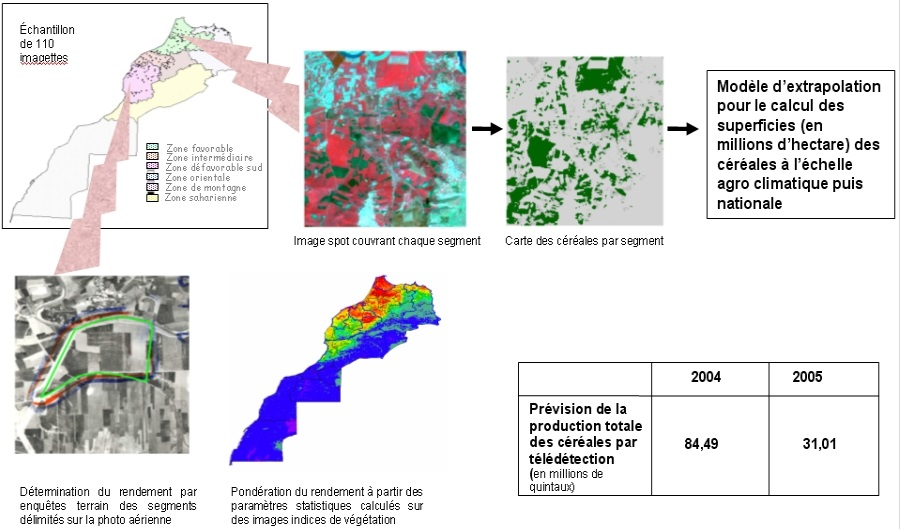
\includegraphics[scale=0.65]{prev.jpg}
\caption{Prévision de la production agricole}
\end{figure}\\
L'intérêt d'utiliser des satellites s'explique par leur capacité à  fournir des images multi spectrales de très bonne résolution. Ces images reçues dans plusieurs longueurs d'onde permettent d'estimer des paramètres biophysiques à partir des pixels de l'image que l'on mesure dans plusieurs couleurs de façon à caractériser l'état de la plante.\\
Ce type d'image a supplanté les systèmes antérieurs en démontrant qu'il pouvait prendre en compte l'état réel des cultures et de la croissance de la végétation à l'intérieur des parcelles à différents stades de la pousse.

\section{Crop Mapping}
\subsection{Définition}
C’est une technique en agriculture qui utilise des données GPS pour analyser des variables telles que le rendement des cultures et la teneur en eau dans un champ donné. Il a été développé dans les années 1990 et utilise une combinaison de technologie GPS et de capteurs physiques, tels que des compteurs de vitesse , pour suivre les rendements des cultures, la vitesse de l' élévateur à grains et combiner la vitesse.\\
Ces données produisent une carte des rendements qui peut être utilisée pour comparer la distribution des rendements dans le champ d'une année à l'autre. Cela permet aux agriculteurs de déterminer les zones du champ qui, par exemple, peuvent avoir besoin d'être plus fortement irriguées ou qui ne produisent aucune récolte. Il permet également aux agriculteurs de montrer les effets d'un changement dans les techniques de gestion des champs, d'élaborer des stratégies nutritionnelles pour leurs champs et d'enregistrer le rendement des cultures à utiliser pour obtenir des prêts ou des locataires.

\subsection{Les méthodes de Crop Mapping}
Il y a plusieurs méthodes de Crop Mapping dont:

\subsubsection{La télédétection (remote sensing from space)}
La télédétection offre une méthode sûre et efficace de cueillette d'information dans le but de cartographier le type et de calculer la superficie des cultures.
Les micro-ondes sont sensibles à l'alignement, la structure et la quantité d'eau présente dans les plantes et dans le sol, et peuvent fournir de l'information complémentaire aux données optiques. \\
Les résultats de l'interprétation des données de télédétection peuvent être intégrés dans un système d'information géographique (SIG) et dans un système de gestion des cultures, et peuvent aussi être combinés à des données auxiliaires pour fournir de l'information sur les droits de propriété, les pratiques de gestion, etc. \hyperref[sec:refs]{7}

\begin{figure}[hp]
\centering
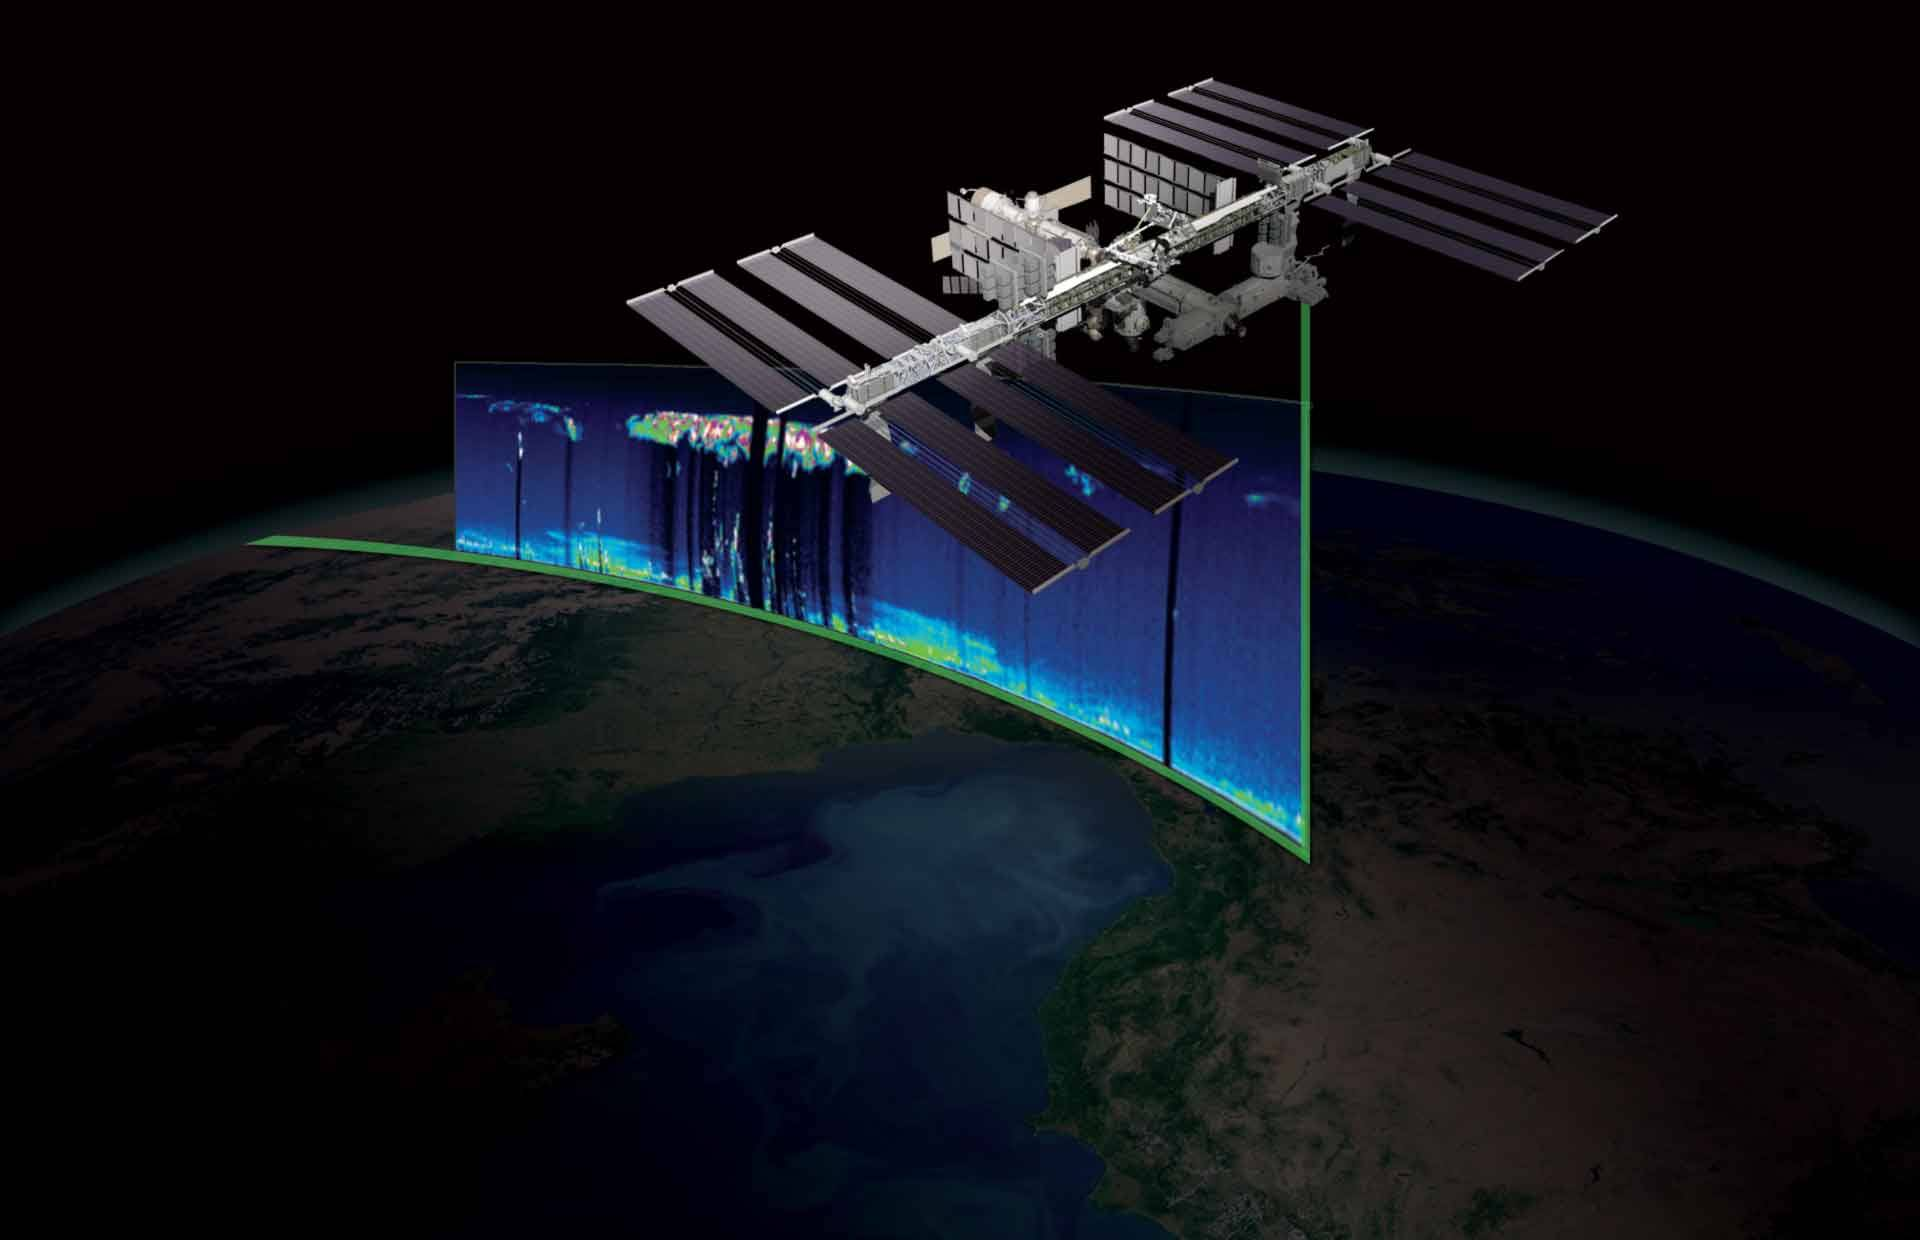
\includegraphics[scale=0.2]{tele.jpg}
\caption{La télédétection par satellite}
\end{figure}

\newpage
\subsubsection{MODIS (Moderate Resolution Imaging Spectroradiometer)}
MODIS est un instrument clé à bord des satellites Terra et Aqua qui sont en orbite de la terre et qui visualise la totalité de sa surface tous les 1 à 2 jours, acquérant des données dans 36 bandes spectrales.\\

\begin{figure}[hp]
\centering
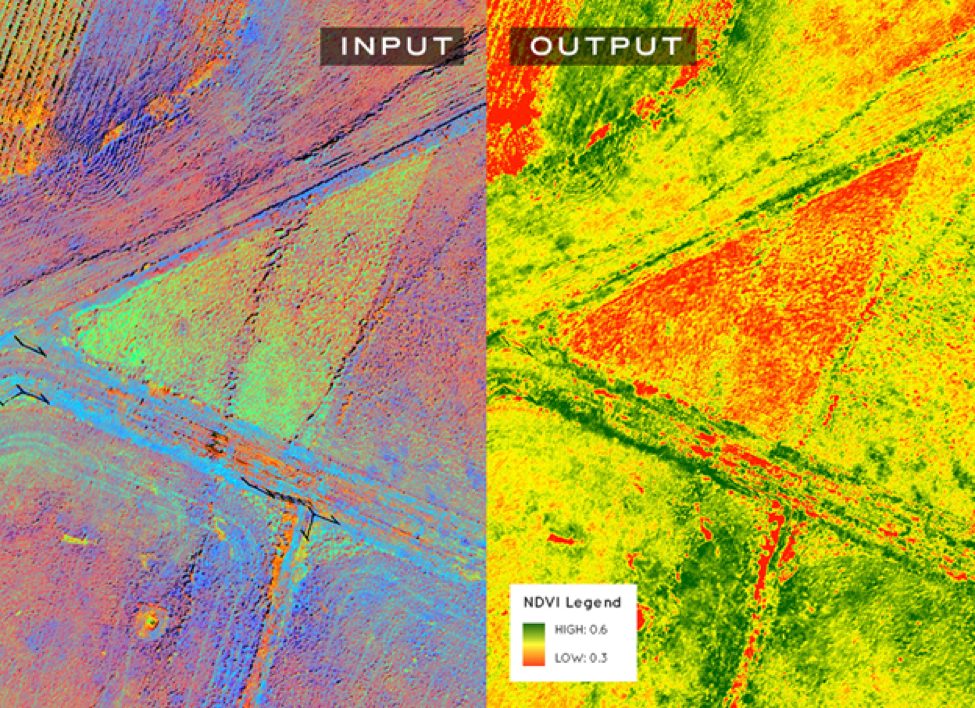
\includegraphics[scale=0.4]{modis.png}
\caption{Une comparaison Input/Output par la méthode MODIS}
\end{figure}

MODIS présente deux indices de végétation (NDVI et EVI) qui fournissent des comparaisons spatiales et temporelles des différentes surfaces à couvert végétale et foliaire, le NDVI (normalized difference vegetation index) assure la continuité de la série temporelle pour des applications historiques et climatiques tandis que le EVI minimise les variations de la canopée et améliore la sensibilité aux conditions de végétation dense.
Ces deux indices caractérisent plus efficacement la gamme mondiale des états et des processus de végétation. \hyperref[sec:refs]{8}


\subsubsection{Deep Learning Classification}
Le Deep Learning (DL) est une technique de pointe puissante pour le traitement d'image, y compris les images de télédétection (remote sensing images). 
Pour cibler la couverture des sols et la classification des types de cultures à partir d'images satellites multi-temporelles et multi-sources, une architecture DL à plusieurs niveaux solide doit être disposer. 
Le pilier de cette architecture est un réseau neuronal qui est utilisé pour la segmentation des images optiques et la restauration des données manquantes en raison des nuages et des ombres. \hyperref[sec:refs]{9} \\

L’avantage de cette méthode est d’étudier des modèles de deep learning/machine learning pour la « crop classification » qui fournissent une segmentation basée sur les pixels d'une zone d'inspection pendant une période donnée. Pour obtenir de meilleurs résultats, il est préférable d’utiliser des modèles existant et de sélectionner ceux les mieux adaptés à la situation. Et pour mieux de flexibilité, il faut ajuster les modèles pré-formés par transfert learning à de nouvelles données comme de nouveaux domaines avec de nouvelles particularités, cultures...\\

\begin{figure}[hp]
\centering
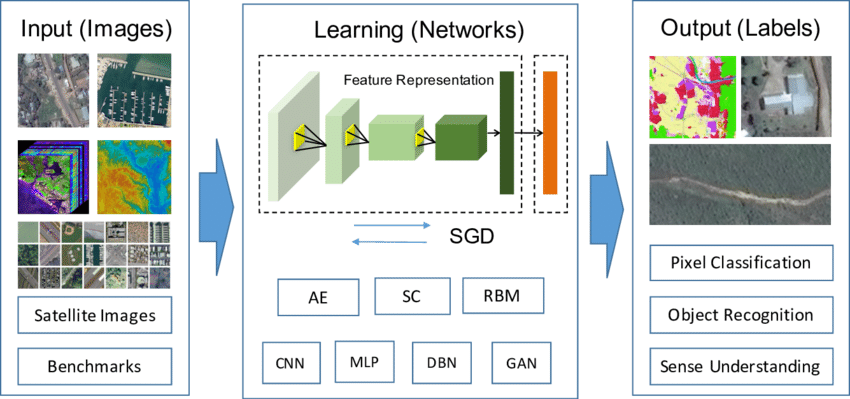
\includegraphics[scale=0.5]{deep.png}
\caption{Le processus de Deep Learning}
\end{figure}

Un autre avantage est le potentiel d'améliorer considérablement la précision d'un modèle avec plus de données réelles recueillies au sol de la région étudié en utilisant des données spécifiques. Cependant, il est possible d'obtenir de meilleurs résultats avec l'ensemble de données de formation (training data set) plus spécifiques.

\chapter*{Bibiographie et Webographie}
\label{sec:refs}
\addcontentsline{toc}{chapter}{Bibliographie et Webographie}
\begin{description}

\item{[1]} La définition de la parcelle est disponible sur:
\\ https://fr.wikipedia.org/wiki/Parcelle

\item{[2]} La fragmentation du parcelle:
\\ http://www.agriculturebiodiversite.fr/ameliorer-la-biodiversite/amenager-son-exploitation\\/fragmentation-du-parcellaire.html

\item{[3]} Les types d'agricultures :
\\ https://www.dev.scienceenlivre.org/index.php/2017/06/28/les-differentes-agricultures/

\item{[4]}  Les images et les statistiques concernat le maroc sont disponible sur:
\\ https://www.crts.gov.ma/thematiques/agriculture

\item{[5]} La définition d'une image satellite est disponible sur:
\\ https://fr.wikiversity.org/wiki/Images\_satellites/Introduction

\item{[6]} Les satellites au service de l'agriculture :
\\ https://www.futura-sciences.com/sciences/actualites/astronautique-satellites-service-agriculture-29034/

\item{[7]} Generating Crop Classification Maps Using AI :
\\ https://www.planetwatchers.com/generating-crop-classification-maps-using-ai/

\item{[8]} La méthode MODIS :
\\ https://modis.gsfc.nasa.gov/data/dataprod/mod13.php

\item{[9]} Deep Learning Classification
\\ https://ieeexplore.ieee.org/abstract/document/7891032?fbclid=IwAR3TiBL273ykf0RpPCO\\RrCK0hayB4ePCgp21eh76O0cBOBMBszCdKtk2E1g


\end{description}

\end{document}








